\documentclass[10pt,oneside,a4paper]{skh-scrreprt}
\title{Software Architecture Draft Proposal}
\subtitle{Neille: A Warstorm-like Card Game Implementation in Lisp}
\author{Sina Khakbaz Heshmati}

\loadglsentries{glossary}

\begin{document}
\maketitle
\tableofcontents
\listoffigures

\chapter{Introduction}\label{chap:intro}

This document is intended 
to outline \emph{an} implementation of
\glsuseri{ws} in \gls{lisp}, 
codenamed \gls{neille}. 
\gls{ws} is a collectible card 
game that is distributed as 
a proprietary software application 
on \glsuseri{facebook}.

\section{Project Scope}\label{sec:scope}

\index{\gls{neille}}
\index{\gls{neille}!goal}
\index{\gls{neille}!scope}
\index{\gls{racket}}
\index{Vrije Universiteit Brussel}

As an advanced programming exercises for 
Computer Science majors at
Vrije Universiteit 
Brussel\footnote{\url{http://www.vub.ac.be/}}, 
the goal of \glsuseri{neille} is to 
provide a graphical environment for
playing \glsuseri{ws}. The code for 
the project must be run on 
\glsuseriii{racket}. 
In addition, 
an artifitial component should also 
be trained to play against human players. 
As part of the project assignment, 
\glsuserii{jpegbd} should also be 
implemented to decode still images 
such as game cards.

\section{About this Document}\label{meta}

This section is intended to give a quick 
overview of the purpose and organization
of this document.

\subsection{Purpose}

The goal of this document 
is to propose a possible 
architecture for a
\gls{ws}-like card game.
At the time of this writing, we may or 
may not have implemented all
the design choices discussed in this document. 
In that sense, this document is a draft proposal 
for building its target software system
and its content is subject to change of 
variable magnitude.

\subsection{Structure}

\index{How to!read this document}

Each chapter in this document is intended to
address a standalone design choice.
The order of the chapters reflects a 
subjective view of the bootstrapping 
process that is hoped to lead to building 
our target software system.
\\

There are multiple ways to browse through this document.
Should you come accross a term that you are not familiar with or
simply seek the intended meaning of a term 
in the context of this document,
please feel free to look up that term in the document 
glossaries \fref{chap:glossaries}.
Additionally, the document index at the end of 
the document may help answer arbitrary queries
as to finding a particular piece of information
inside the document.

\chapter{On Reading Warstorm Cards into Memory}\label{chap:load-ws-cards}

\section{Problem}

\index{\gls{ws}!cards!load into memory}

The issue that 
is addressed 
in this chapter is 
how \gls{ws} cards
are loaded 
into the central memory 
of a computer 
that is running 
\glsuseriv{racket}. 
In other words, 
how are we going 
to make \gls{ws} cards available 
to our program. 
An obvious solution is
to devise an \gls{adt} 
in \gls{racket} 
and \emph{hard code} 
the required cards 
as instances 
of that \gls{adt}. 
The above approach 
has a few key drawbacks, 
including lack of felxibility, 
and error-proneness 
of the encoding process.

\section{Solution}\label{sec:xml-cards-to-racket}

\index{\gls{xml}}
\index{\gls{xslt}}
\index{\gls{xpath}}
\index{\gls{racket}!generate}
\index{\gls{rng}}

The approach that we are going
to propose in this document
is to take advantage of the \gls{xml} toolchain.
The idea is to store \gls{ws} card 
descriptions in an \gls{xml}-based 
high-level language specified for
\gls{ws} cards in \glsuseri{rng}.
Given \gls{ws} cards serialized in \gls{xml},
we can use \gls{xslt} 
and \gls{xpath}
to generate 
\gls{racket} code 
that once evaluated, 
will read card descriptions 
into memory and makes \gls{ws} cards 
available throughout our program.

\begin{figure}[h]\label{fig:cards-to-racket}
\caption[Transform Warstorm Card Descriptions from XML into Lisp]{%
The process that transforms Warstorm card descriptions conforming
to a high-level XML grammar into Lisp}
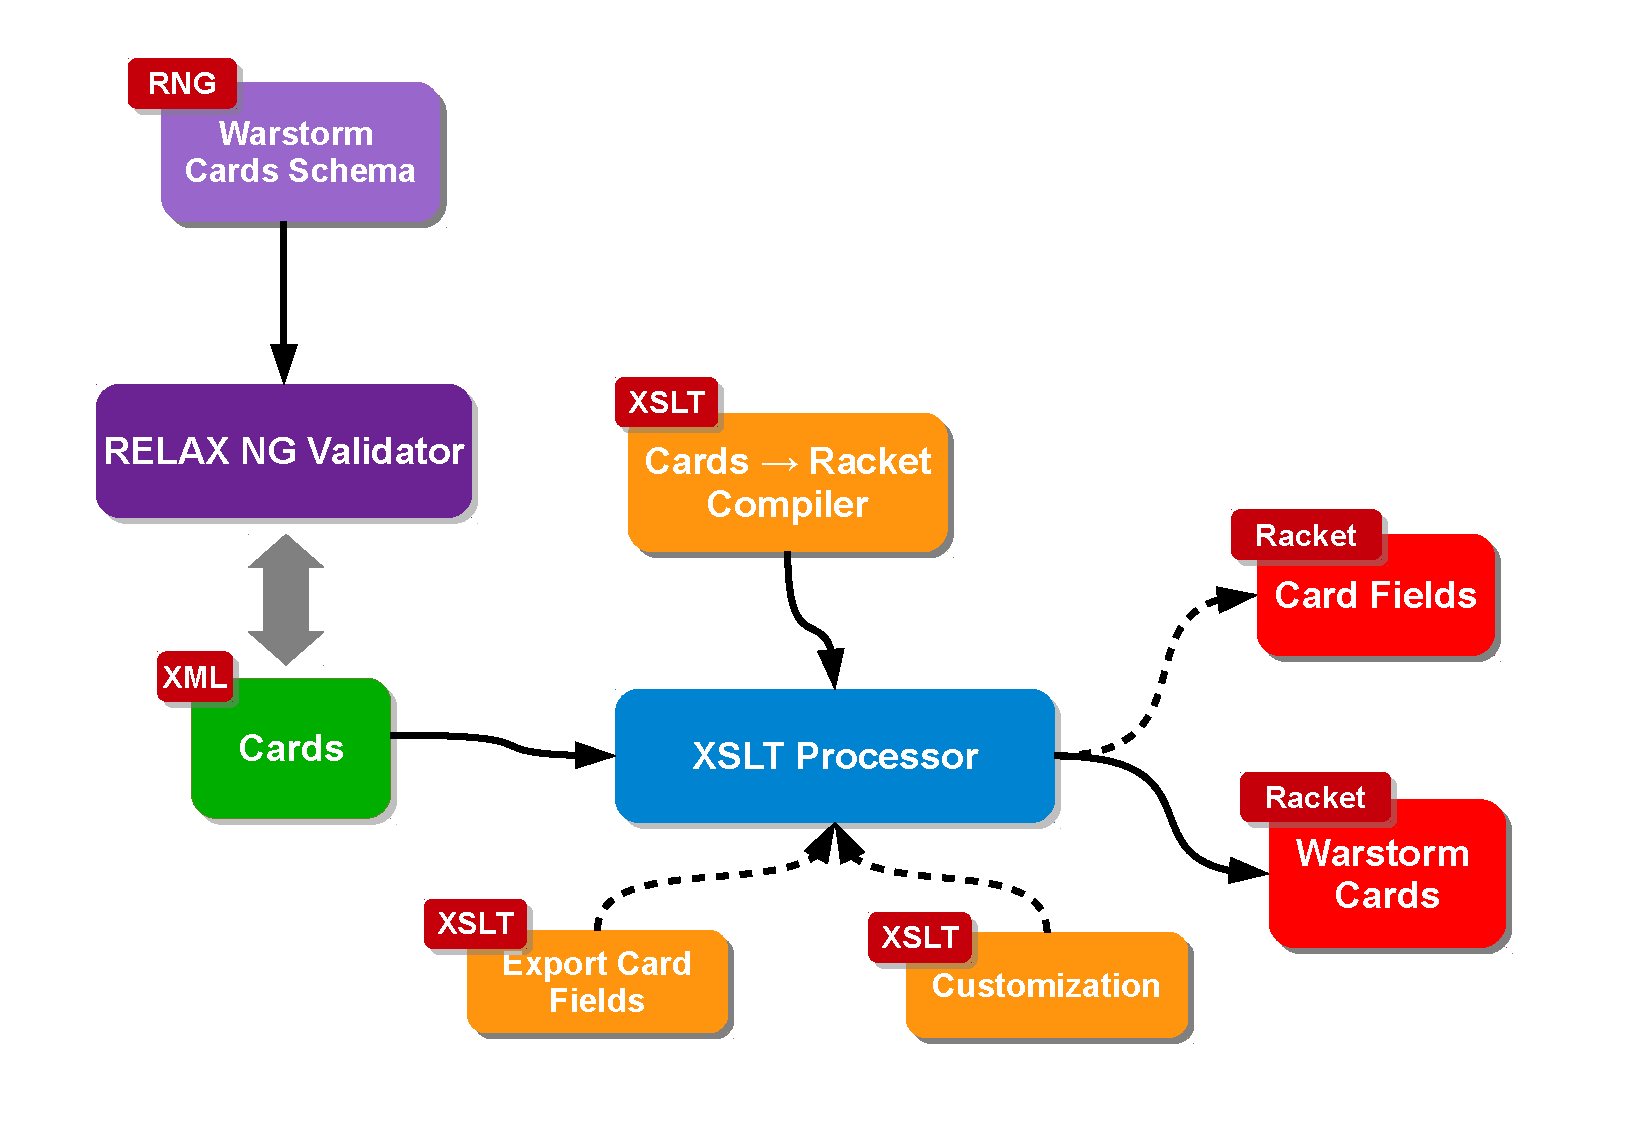
\includegraphics[width=14cm]{fig/cards-to-racket}
\end{figure}

\index{\gls{ws}!cards!load into memory!diagram}
\Fref{fig:cards-to-racket} depicts 
the process that reads the description
of \gls{ws} cards from \gls{xml} source
and generates the necessary \gls{racket}
code to make the input cards
available in \glsuseriii{racket}.
The \emph{Cards to Racket Compiler}
component is the \glsuservi{xslt}
that performs the main transformation.
\emph{Customization} helps control
the \gls{racket} output generated by the
set of stylesheets.
The \emph{Export Card Fields} component
produces the necessary information
to be able to automatically
generate accessors and mutators
for \gls{ws} card objects.
The \emph{Cards} component refers to
the XML document that contains
\gls{ws} card descriptions
(\fref{chap:cards-in-xml})
and \emph{\gls{ws} Cards Schema}
refers to the grammar against
which \gls{xml} card definitions
must validate.

\subsection{Source Preparation}

An example 
of a collectible card
expressed in our 
\gls{xml}-based language
for \gls{ws} cards is shown in 
\fref{fig:sample-card-in-xml}.
Please note that
we can either choose 
to encode card descriptions 
directly in \gls{xml} 
or generate an \gls{xml} document
by reading an already-existing
database of card descriptions. 
The point however remains the same. 
Once the card descriptions 
are encoded in \gls{xml}, 
the validation process against 
the grammar specified for \gls{ws} cards
(\fref{chap:ws-card-vocab}) can verify the 
correctness of card descriptions.

\begin{figure}[h]\label{fig:sample-card-in-xml}
\caption[Sample Warstorm Card in XML Format]{%
A sample card defined in a high-level XML vocabulary}
\lstinputlisting[language=XML]{fig/sample-card.xml}
\end{figure}

In addition to ensured correctness of 
encoded cards, specifying \gls{ws} 
cards in \gls{xml} has a number of 
other advantages, 
including but not limited to:
\begin{itemize}
\item Persistent storage of \gls{ws} cards 
  in a format that is both
  human and machine-readable.
\item 
  \index{\gls{xml}}
  \index{\gls{xslt}}
  \index{\gls{xpath}}
  Once in \gls{xml}, the information can
  undergo any processing step with minimal effort.
  Technologies that help process \gls{xml} include
  \gls{xslt} and \gls{xpath}.
\item
  \index{\gls{nxml}}
  Easy authoring and maintenance of card descriptions
  with schema-aware \gls{xml} editors --e.g. \gls{nxml}.
\item Hassle-free, unambiguous, and cross-application 
  exchange of \gls{ws} cards.
\end{itemize}

\subsection{Lisp Generation}

Assuming that we have an \gls{xml} 
\emph{document} that contains \gls{ws} 
card descriptions and is compliant with
the grammar specified in \fref{chap:ws-card-vocab}
for \gls{ws} cards, we can process this document
to generate \gls{racket} code that once run,
will load \gls{ws} cards into 
the central memory of a computer that is
running \gls{racket}.
\Fref{fig:sample-card-in-racket} shows a
\gls{racket} code snippet that can be generated,
given the \gls{xml} definition of the
\gls{ws} card specified in \fref{fig:sample-card-in-xml}.

\begin{figure}[h]\label{fig:sample-card-in-racket}
\caption[Warstorm Card Definition in Racket Generated from XML]{%
  A sample Warstorm card definition in Racket that is generated from XML
  source}
\lstinputlisting[language=Lisp]{fig/sample-card.rkt}
\end{figure}

\section{Solution Outline}

The solution that we have proposed in 
\fref{sec:xml-cards-to-racket}
has the advantage of making it
easy to encode cards in a
machine-readable form.
It is also very flexible since
the code that loads \gls{ws} cards into
memory can be adapted at anytime
during the project development,
hence refactoring can be
performed on the output \gls{racket}
code with minimal effort.
A disadvantage, one might argue,
is that there is a disconnect
between the meta level and the
base level. That is, the
\gls{racket}-generating \gls{xslt} is
\gls{racket}-agnostic for \emph{as it is},
it is not checked whether
the generated code is 
\emph{well-formed} and \emph{sound}.
Well-formedness can however
be guaranteed by carefully
building and systematically using
an abstraction layer
between \gls{xslt} and \gls{racket}
but the semantics of the generated
code will only be checked outside
the \gls{xslt} processing unit.
That said, we can easily introduce
an extra step in our
\gls{xml} processing pipeline
to run the generated code through
\glsuserii{racket} and report
back errors in program's semantics
but this issue is not considered
significant and doing so falls beyond the
scope of this project.

\chapter{On Separation of Concerns}\label{chap:soc}

\index{\gls{ws}!semantics}

In this chapter, our goal 
is to show how we are going to
design a system whose
\emph{semantics} are \emph{separate}
from its \emph{presentation}.

\section{Problem}\label{sec:soc-problem}

Let us illustrate the
issue that we are trying to
address in this chapter 
by way of an example.
Consider a deck of cards
in our game, which is very
similar to the stack
data structure.
For instance, dealing a 
card from a deck
is equivalent to popping
an element from a stack.
Now, the question is:
can a deck be represented
by only a stack?
The answer is:
it takes more than just
a stack to represent
a card deck, given
the requirements of our system,
which include giving feedback
to the user upon changes
in the state of the game.
So we can view a deck as an abstraction
that has two responsibilities.
First to maintain its
internal state --\emph{semantics}--
in this case, represented by a stack,
and second, to report 
back the changes in its state
to the human player 
--\emph{presentation}.
In the interest of brevity,
game abstractions that purely
represent the game semantics
are referred to
as \emph{models} and \emph{views}
refer to abstractions
that keep the presentation
up-to-date.
\\

Our goal is to separate these
two responsibilities so that 
views are merely loosely coupled
to models.
In other words, we want
to make sure that models
are presentation-agnostic.
There are several reasons
why we would like to keep
these two aspects separate;
here, we list a few of them:

\begin{itemize}
\item
  We would like the logic of the game
  to be expressed as clearly as possible, 
  and not cluttered with presentational 
  instructions.
\item
  For training the robot player
  and unit testing of abstractions,
  the graphical presentation 
  should be switched off, which can
  easily be done when the presentational
  aspect is isolated.
\item
  Should the separation
  of concerns be respected,
  several, and possibly simultaneous
  feedback mechanisms could
  be put in place on-the-fly,
  without having to alter
  the implementation of models.
\end{itemize}

\section{Solution}\label{sec:soc-solution}

\def \cardlist{\texttt{CardList}}
\def \deck{\texttt{Deck}}
\def \model{\texttt{Model}}
\def \view{\texttt{View}}
\def \region{\texttt{Region}}
\def \observer{\texttt{Observer}}
\def \notify{\texttt{notify}}
\def \update{\texttt{update}}
\def \subviews{\texttt{subviews}}

\index{\glsname{mvc}}
\begin{figure}[h]\label{fig:mvc}
\caption[%
Object-oriented Structure of
a Reactive System for Neille
]{%
A model that captures 
a reactive system to achieve 
separation of concerns
between two aspects
of game components. 
One aspect is represented by
model components
and they caputure 
pure semantics of the game.
The other aspect is 
the feedback mechanism 
that reports back
changes in the state of 
the game by way of
the graphical user interface
and is represented by view components}
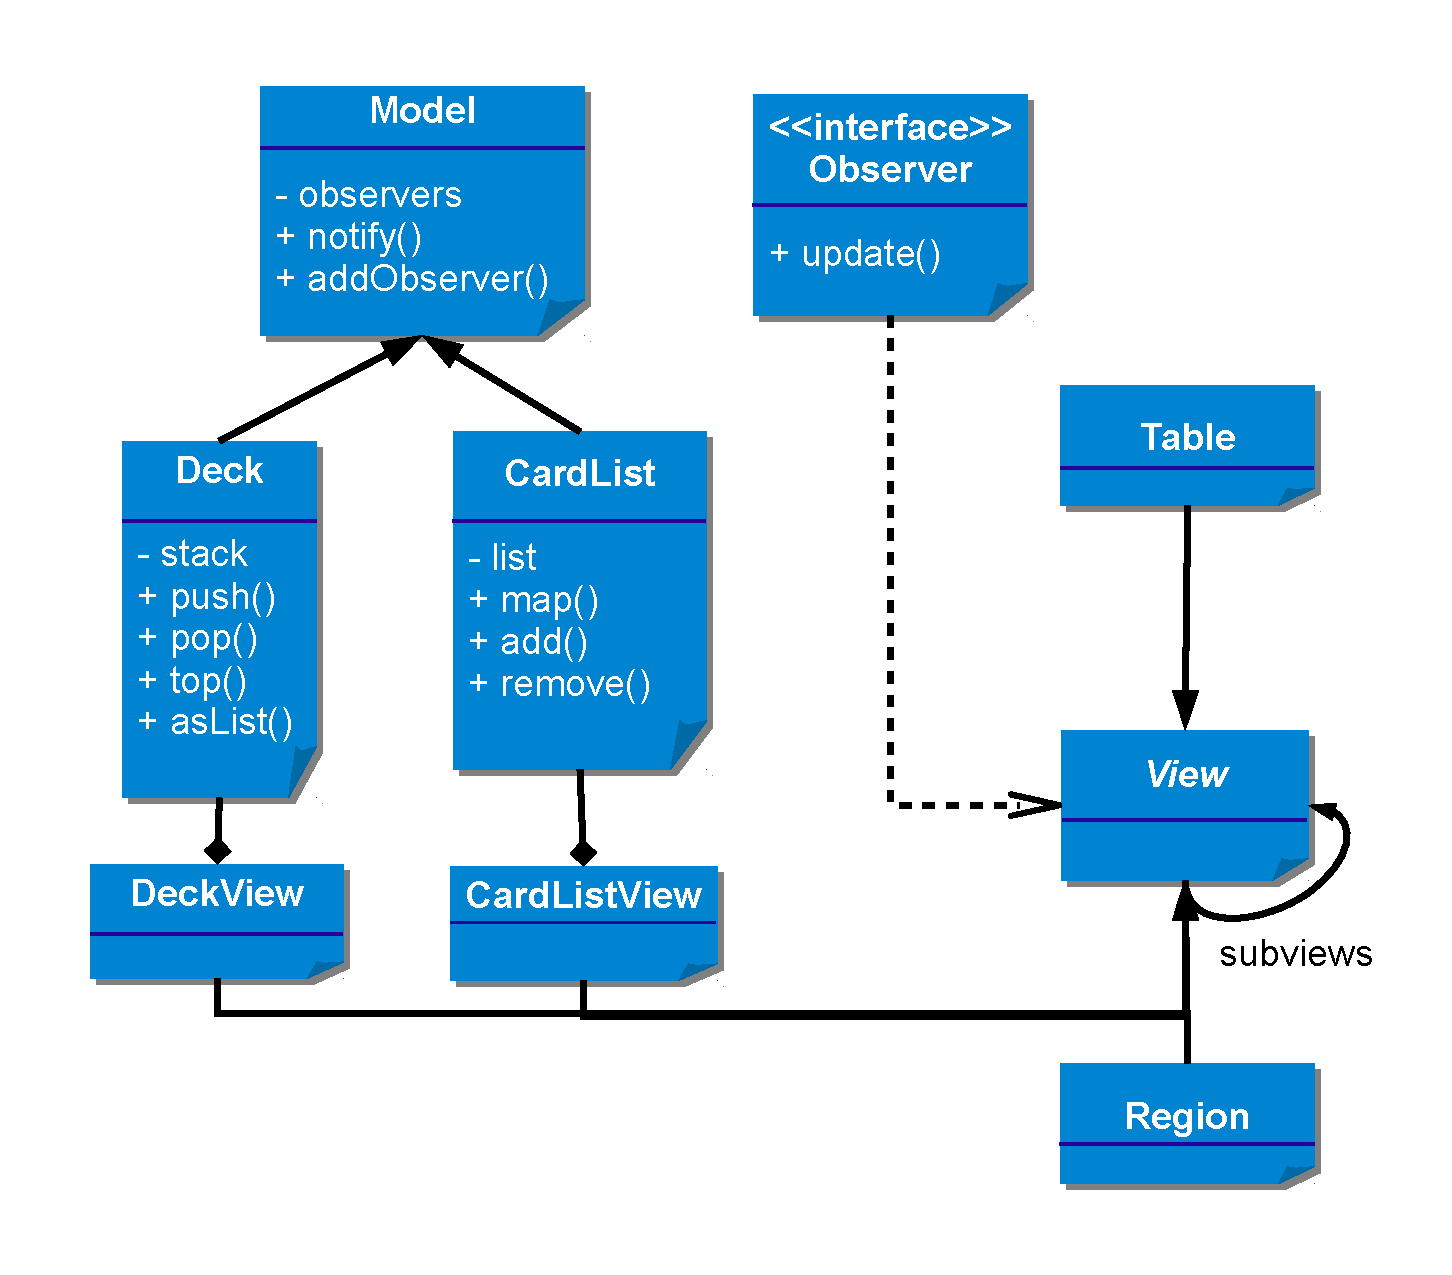
\includegraphics[width=15.5cm]{fig/class-structure}
\end{figure}

The problem that
we would like to
address in this
chapter, as established
in \fref{sec:soc-problem}
is to separate
models from views in
such a way that models
purely represent the
game semantics
and views would be
separate mechanisms that
react to changes in models.
In order to put in place
a reactive system,
we are going to propose
a direct application of
the \gls{mvc} design pattern.
\\

\Fref{fig:mvc} attempts
to model a reactive system
that achieves separation
of concerns in our program.
\cardlist{} and \deck{} 
are subclasses of \model{}.
\model{} maintains a
list of objects that
implement the \observer{}
interface.
Upon changes in
the state of a
model --e.g. \deck{},
the model
sends a \notify{}
message to itsef, the
implementation of which
is provided by its
parent, i.e. \model{}.
The \notify{} method
simply traverses the list
of observers and sends
the \update{} message
to each observer.
As we can see in the 
diagram, views must
all implement the
\update{} method by
way of the \observer{}
interface. Hence,
the workflow
can be layed out
as follows:
a \view{} object is 
initialized with instances of
\model{} and \region{} classes
and an optional list of \subviews{}
as its state.
After our view registers
itself to observe its model,
its \update{} method will
be invoked when changes
occur in the model it watches.
It is now up to the view
to reflect the changes to the
human player by altering the
elements of \glsuseri{gui},
to which it has access throug
the \region{} object.

\section{Solution Outline}

\index{Reavtive System!implementation}
\index{\glsname{gui}}
\index{Callback}

An alternative solution
to the one presented in
\fref{sec:soc-solution}
is to have state-altering
methods of a model
receive an extra callback
procedure as parameter.
These methods can then
apply the callback
procedure they have received
as soon as they will have
altered the state of
their parent model.
This mechanism is
elegent and
straightforward to 
put in place in languages
such as \gls{racket}
that treat procedures
as first-class citizens.
The reason why we
did not choose the
ad-hoc callback approach 
is that doing so requires
extra overhead in order to
orchestrate the various
callback procedures
that will be passed
as arguments to models.
For instance,
we need to make sure
to equip the lexical
environment of callback
procedures with objects
that might be needed
while computing the reaction
to the event that caused the
callback procedure to be applied
in the first place.
\index{\glsname{mvc}}
We prefer to apply \glsuseri{mvc}
in this case because of the clean
organization \gls{mvc} gives
to different components of
the program.

\chapter{On Making Graphical Interfaces}\label{chap:gui}

\index{\glsname{gui}}

%% The topic 
%% that we are going
%% to discuss
%% in this chapter
%% is how
%% the graphical interactions
%% or \glsuseriii{gui}
%% is built 
%% in our program.

%% \section{Problem}\label{sec:gui-problem}

%% \section{Solution}\label{sec:gui-solution}

\begin{figure}[h]\label{fig:layout-to-racket}
\caption{XML Layout to Racket Compiler}
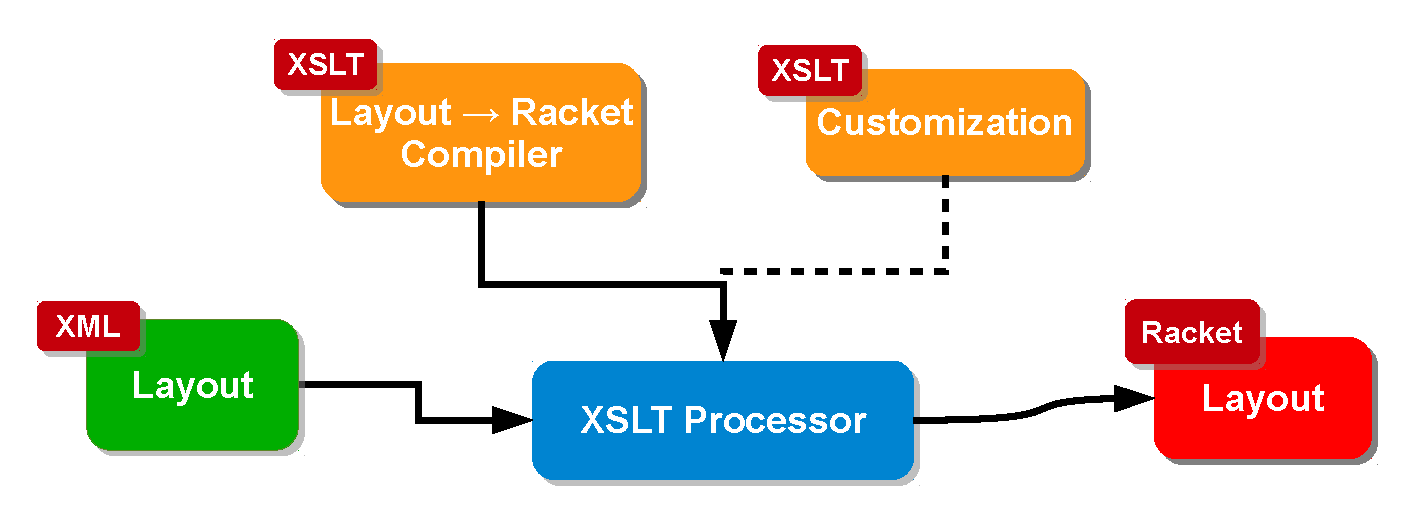
\includegraphics[width=14cm]{fig/layout-to-racket}
\end{figure}

%% \section{Solution Outline}

\chapter{On Representing Structured Data}

%% \section{Card}

%% \section{Player}

%% \section{Deck}

%% \section{Card Collection}

\chapter{On Representing Processes}

\section{Card Abilities}

\chapter{On Persistent Storage of Players' History}

\chapter{On Designing an Artificial Player}
\gls{ai}
\chapter{On Decoding JPEG Images}

\appendix

\chapter{Warstorm Cards in XML}\label{chap:cards-in-xml}
\index{\gls{ws}!cards!in \gls{xml} format}
\lstinputlisting[language=XML]{fig/neille/cards/cards.xml}

\chapter{XML Grammar for Warstorm Cards}\label{chap:ws-card-vocab}

\index{\gls{ws}!cards!XML grammar}

\section{Card Collection}
\lstinputlisting{fig/neille/cards/schema/cards.rnc}

\section{Card}
\lstinputlisting{fig/neille/cards/schema/card.rnc}

\section{Enumerations}
\lstinputlisting{fig/neille/cards/schema/enums.rnc}

\section{Common Definitions}
\lstinputlisting{fig/neille/cards/schema/common.rnc}

\chapter{User Interface Layout Definitions}

\section{UI Layout for Battle}
\lstinputlisting[language=XML]{fig/neille/battle/layout/layout.xml}

\chapter{Definitions and Terms}\label{chap:glossaries}
\printglossaries

\addcontentsline{toc}{chapter}{Revision History}
\begin{versionhistory}
  \vhEntry{0.1.0}{2011-08-22}{SKH}{%
    Early draft sent for review}
  \vhEntry{0.1.1}{2011-08-25}{SKH}{%
    First draft published}
\end{versionhistory}

\addcontentsline{toc}{chapter}{Index}
\printindex

\addcontentsline{toc}{chapter}{References}
\cite{bray_namespaces_2009}
\cite{bray_extensible_2008}
\cite{burbeck_applications_1987}
\cite{fokker_functional_1995}
\cite{clark_xml_1999}
\cite{clark_xsl_1999}
\cite{clark_relax_2002}
\cite{clark_relax_2002-1}
\cite{dijkstra_role_1982}
\cite{kobayashi_scheme_2006}
\cite{flatt_reference:_2011}
\cite{flatt_gui:_2011}
\cite{gamma_design_1995}
\cite{international_telecommunication_union_information_1993}

\bibliographystyle{plain}\label{sec:refs}
\bibliography{main}

\end{document}
